\documentclass{article}

\usepackage{amsmath}
\usepackage{graphicx}
\usepackage{enumitem}

\title{CEM3350 Analysis}
\author{Guy John \\ \texttt{guy@rumblesan.com}}

\begin{document}

\maketitle

\section{Introduction}
A verbose but hopefully useful and correct analysis of the CEM3350 and AS3350 VCF IC\@. An input can be sent to multiple places within the circuit to obtain different responses and gains. Either a LowPass/BandPass response or a BandPass/HighPass response can be created. The input can also be sent to a fixed or variable gain input or some mix of the two. This will control the level of the output as the Q increases.

\begin{figure}[h]
  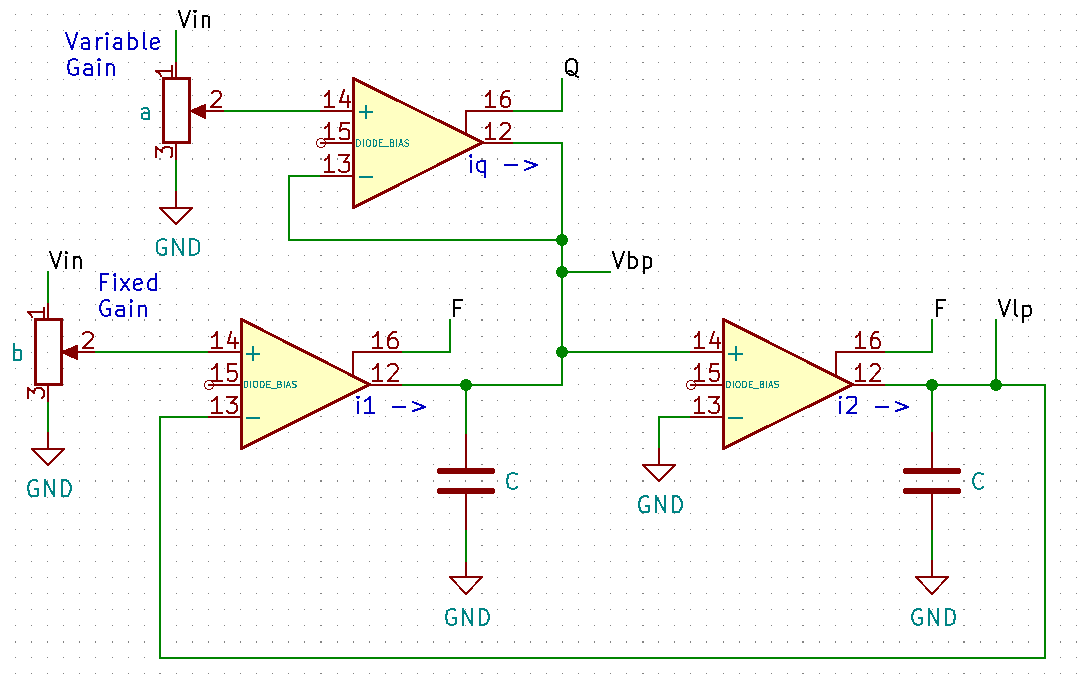
\includegraphics[width=\linewidth]{lpbp.png}
  \caption{LowPass/BandPass configuration}
\end{figure}

\newpage

\subsection{Notations}

\begin{description}
\item[F] is the the frequency control variable
\item[Q] is the the Q control variable
\item[a] is the variable gain input scaling factor
\item[b] is the fixed gain input scaling factor
\end{description}

\section{LowPass/BandPass Configuration}

\begin{equation}
  iq = Q(aV_{in} - V_{bp})
\end{equation}


\begin{equation}
  i1 = F(bV_{in} - V_{lp})
\end{equation}

\begin{equation}
  i2 = FV_{bp}
\end{equation}

\begin{equation}
  \hat{V}_{bp} = \frac{\hat{I}_1 + \hat{I}_q}{sC}
\end{equation}

\begin{equation}
  \hat{V}_{lp} = \frac{\hat{I}_2}{sC}
\end{equation}

Simplify Vbp into terms of Vlp and Vin.

\begin{equation*}
\begin{split}
  \hat{V}_{bp} & = \frac{\hat{I}_1 + \hat{I}_q}{sC} \\
  sC\hat{V}_{bp} & = \hat{I}_1 + \hat{I}_q \\
  sC\hat{V}_{bp} & = Fb\hat{V}_{in} - F\hat{V}_{lp} + Qa\hat{V}_{in} - Q\hat{V}_{bp} \\
  sC\hat{V}_{bp} + Q\hat{V}_{bp} & = Fb\hat{V}_{in} - F\hat{V}_{lp} + Qa\hat{V}_{in}\\
  \hat{V}_{bp}(sC + Q) & = \hat{V}_{in}(Fb + Qa) - F\hat{V}_{lp} \\
\end{split}
\end{equation*}

\begin{equation}
  \hat{V}_{bp} = \frac{\hat{V}_{in}(Fb + Qa) - F\hat{V}_{lp}}{sC + Q}
\end{equation}

Get Vlp in terms of Vin and calculate Low Pass transfer function.

\begin{equation*}
\begin{split}
  \hat{V}_{lp} & = \frac{\hat{I}_2}{sC} \\
  \hat{V}_{lp} & = \frac{F\hat{V}_{bp}}{sC} \\
  sC\hat{V}_{lp} & = F\hat{V}_{bp} \\
  sC\hat{V}_{lp} & = \frac{\hat{V}_{in}(F^2b + FQa) - F^2\hat{V}_{lp}}{sC + Q} \\
  \hat{V}_{lp}(s^2C^2 + sCQ) & = \hat{V}_{in}(F^2b + FQa) - F^2\hat{V}_{lp} \\
  \hat{V}_{lp}(s^2C^2 + sCQ) + F^2\hat{V}_{lp} & = \hat{V}_{in}(F^2b + FQa) \\
  \hat{V}_{lp}(s^2C^2 + sCQ + F^2) & = \hat{V}_{in}(F^2b + FQa) \\
  \frac{\hat{V}_{lp}}{\hat{V}_{in}} & = \frac{F^2b + FQa}{s^2C^2 + sCQ + F^2} \\
  & = \frac{b + a\frac{Q}{F}}{s^2{(\frac{C}{F})}^2 + s\frac{C}{F}\frac{Q}{F} + 1} \\
\end{split}
\end{equation*}

\begin{equation}
  H(s) = \frac{b + a\frac{Q}{F}}{\frac{s^2}{{(\frac{F}{C})}^2} + 2\frac{s}{\frac{F}{C}}\frac{Q}{2F} + 1}
\end{equation}

Calculate Band Pass transfer function.

\begin{equation*}
\begin{split}
  \hat{V}_{bp} & = \frac{\hat{V}_{in}(Fb + Qa) - F\hat{V}_{lp}}{sC + Q} \\
  \hat{V}_{bp}(sC + Q) & = \hat{V}_{in}(Fb + Qa) - F\hat{V}_{lp} \\
  \hat{V}_{bp}(sC + Q) & = \hat{V}_{in}(Fb + Qa) - \frac{F^2\hat{V}_{bp}}{sC} \\
  \hat{V}_{bp}(s^2C^2 + sCQ) & = sC\hat{V}_{in}(Fb + Qa) - F^2\hat{V}_{bp} \\
  \hat{V}_{bp}(s^2C^2 + sCQ) + F^2\hat{V}_{bp} & = sC\hat{V}_{in}(Fb + Qa) \\
  \hat{V}_{bp}(s^2C^2 + sCQ + F^2) & = sC\hat{V}_{in}(Fb + Qa) \\
  \frac{\hat{V}_{bp}}{\hat{V}_{in}} & = \frac{sC(Fb + Qa)}{s^2C^2 + sCQ + F^2} \\
  & = \frac{s\frac{C}{F^2}(Fb + Qa)}{s^2\frac{C^2}{F^2} + s\frac{CQ}{F^2} + 1} \\
  & = \frac{s\frac{C}{F}{(b + \frac{Q}{F}a)}}{s^2{(\frac{C}{F})}^2 + s\frac{Q}{F}\frac{C}{F} + 1} \\
\end{split}
\end{equation*}

\begin{equation}
  H(s) = \frac{s\frac{C}{F}{(b + \frac{Q}{F}a)}}{\frac{s^2}{{(\frac{F}{C})}^2} + 2\frac{s}{\frac{F}{C}}\frac{Q}{2F} + 1} \\
\end{equation}

\end{document}
